\documentclass{exam}
\usepackage{mainExam}

\title{Évaluation de cours}
\author{Seconde 9}
\date{21 Mars 2025}

\begin{document}
\maketitle

\begin{questions}
\question 
\hfill
% \vspace*{0.4cm}
\begin{tcolorbox} 
Soit $f$ une fonction définie sur $[-5;5]$. Pour chaque courbe représentative $\mathcal{C}_f$ donnée ci-après, résoudre l'équation ou l'inéquation qui lui est associée. On fera apparaître les traits de construction nécessaires. Puis, on donnera $\mathcal{S}$ l'ensemble des solutions de l'équation ou inéquation donnée (ou l'écrire en français sinon).
\end{tcolorbox}
\begin{minipage}{0.4\textwidth} 
\begin{equation*}
f(x) \geq 2
\end{equation*}
\begin{center}
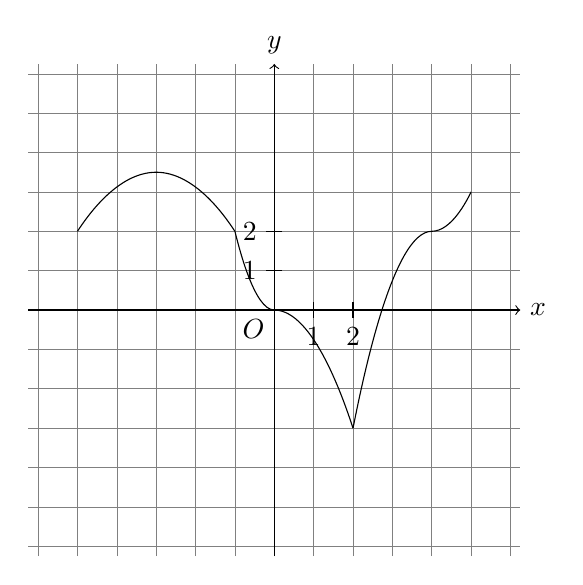
\begin{tikzpicture}[scale=0.5]
\draw[help lines] (-6.25,-6.25) grid (6.25,6.25);
\draw[->] (-6.25,0) -- (6.25,0) node[right] {$x$};
\draw[->] (0,-6.25) -- (0,6.25) node[above] {$y$};
\foreach \x in {1,2}
    {\draw (\x,0.2)--(\x,-0.2) node[below] {$\x$};}
\foreach \y in {1,2}
    {\draw (0.2,\y)--(-0.2,\y) node[left] {$\y$};}
\draw (0,0) node[below left] {$O$};
\draw (-5,2) parabola bend (-3,3.5) (-1,2);
\draw (-1,2) parabola[bend at end] (0,0);
\draw (0,0) parabola (2,-3);
\draw (2,-3) parabola bend (4,2) (5,3);
\end{tikzpicture}
\end{center}
$\mathcal{S}$ = \answersline
\vspace*{0.5cm}
\begin{equation*}
f(x) = -3
\end{equation*}
\begin{center}
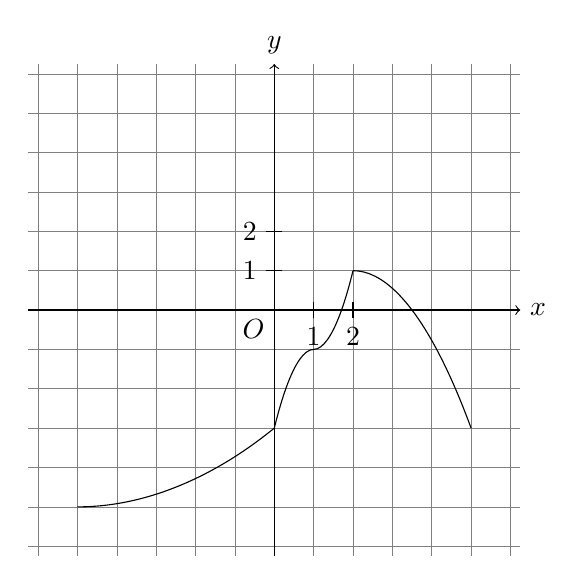
\begin{tikzpicture}[scale=0.5]
\draw[help lines] (-6.25,-6.25) grid (6.25,6.25);
\draw[->] (-6.25,0) -- (6.25,0) node[right] {$x$};
\draw[->] (0,-6.25) -- (0,6.25) node[above] {$y$};
\foreach \x in {1,2}
    {\draw (\x,0.2)--(\x,-0.2) node[below] {$\x$};}
\foreach \y in {1,2}
    {\draw (0.2,\y)--(-0.2,\y) node[left] {$\y$};}
\draw (0,0) node[below left] {$O$};
\draw (-5,-5) parabola (0,-3);
\draw (0,-3) parabola bend (1,-1) (2,1);
\draw (2,1) parabola (5,-3);
\end{tikzpicture}
\end{center}
$\mathcal{S}$ = \answersline
\end{minipage}
\hfill
\begin{minipage}{0.4\textwidth}
\begin{equation*}
f(x) = 1
\end{equation*}
\begin{center}
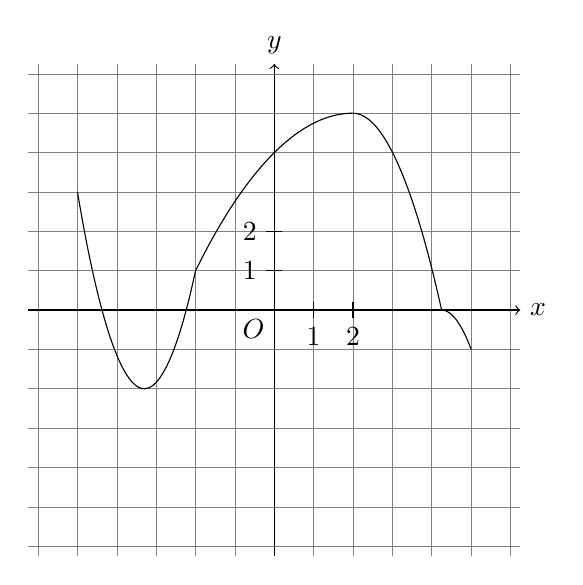
\begin{tikzpicture}[scale=0.5]
\draw[help lines] (-6.25,-6.25) grid (6.25,6.25);
\draw[->] (-6.25,0) -- (6.25,0) node[right] {$x$};
\draw[->] (0,-6.25) -- (0,6.25) node[above] {$y$};
\foreach \x in {1,2}
    {\draw (\x,0.2)--(\x,-0.2) node[below] {$\x$};}
\foreach \y in {1,2}
    {\draw (0.2,\y)--(-0.2,\y) node[left] {$\y$};}
\draw (0,0) node[below left] {$O$};

\draw (-5,3) parabola bend (-3.3,-2) (-2,1);
\draw (-2,1) parabola bend (2,5) (4.25,0);
\draw (4.25,0) parabola (5,-1);
\end{tikzpicture}
\end{center}
$\mathcal{S}$ = \answersline
\vspace*{0.5cm}
\begin{equation*}
f(x) < -2
\end{equation*}
\begin{center}
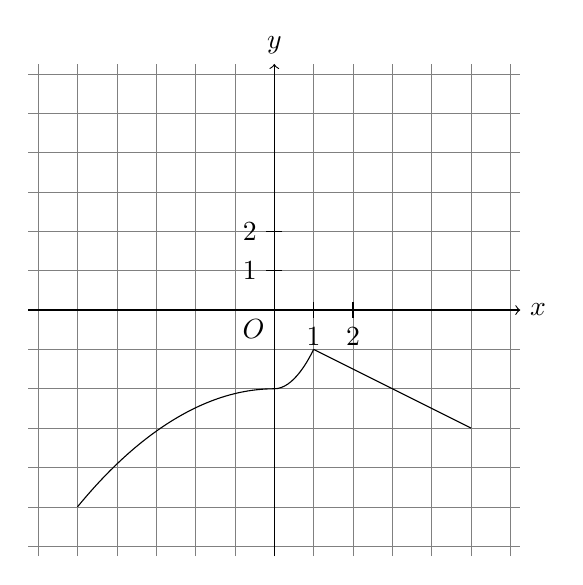
\begin{tikzpicture}[scale=0.5]
\draw[help lines] (-6.25,-6.25) grid (6.25,6.25);
\draw[->] (-6.25,0) -- (6.25,0) node[right] {$x$};
\draw[->] (0,-6.25) -- (0,6.25) node[above] {$y$};
\foreach \x in {1,2}
    {\draw (\x,0.2)--(\x,-0.2) node[below] {$\x$};}
\foreach \y in {1,2}
    {\draw (0.2,\y)--(-0.2,\y) node[left] {$\y$};}
\draw (0,0) node[below left] {$O$};

\draw (-5,-5) parabola bend (0,-2) (1,-1);
\draw (1,-1) -- (5,-3);
\end{tikzpicture}
\end{center}
$\mathcal{S}$ = \answersline
\end{minipage}
\end{questions}
\newpage

\maketitle

\begin{questions}
\question 
\hfill
% \vspace*{0.4cm}
\begin{tcolorbox} 
Soit $f$ une fonction définie sur $[-5;5]$. Pour chaque courbe représentative $\mathcal{C}_f$ donnée ci-après, résoudre l'équation ou l'inéquation qui lui est associée. On fera apparaître les traits de construction nécessaires. Puis, on donnera $\mathcal{S}$ l'ensemble des solutions de l'équation ou inéquation donnée.
\end{tcolorbox}
\begin{minipage}{0.4\textwidth} 
\begin{equation*}
f(x) \geq 4
\end{equation*}
\begin{center}
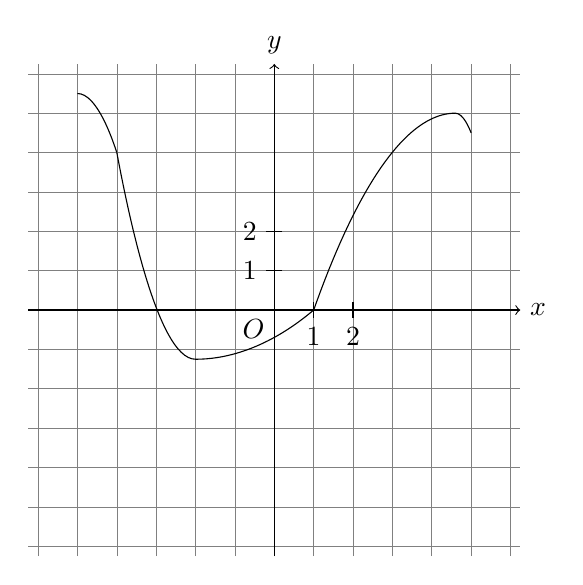
\begin{tikzpicture}[scale=0.5]
\draw[help lines] (-6.25,-6.25) grid (6.25,6.25);
\draw[->] (-6.25,0) -- (6.25,0) node[right] {$x$};
\draw[->] (0,-6.25) -- (0,6.25) node[above] {$y$};
\foreach \x in {1,2}
    {\draw (\x,0.2)--(\x,-0.2) node[below] {$\x$};}
\foreach \y in {1,2}
    {\draw (0.2,\y)--(-0.2,\y) node[left] {$\y$};}
\draw (0,0) node[below left] {$O$};

\draw (-5,5.5) parabola (-4,4);
\draw (-4,4) parabola bend (-2,-1.25) (1,0);
\draw (1,0) parabola bend (4.6,5) (5,4.5);
\end{tikzpicture}
\end{center}
$\mathcal{S}$ = \answersline
\vspace*{0.5cm}
\begin{equation*}
f(x) = 0
\end{equation*}
\begin{center}
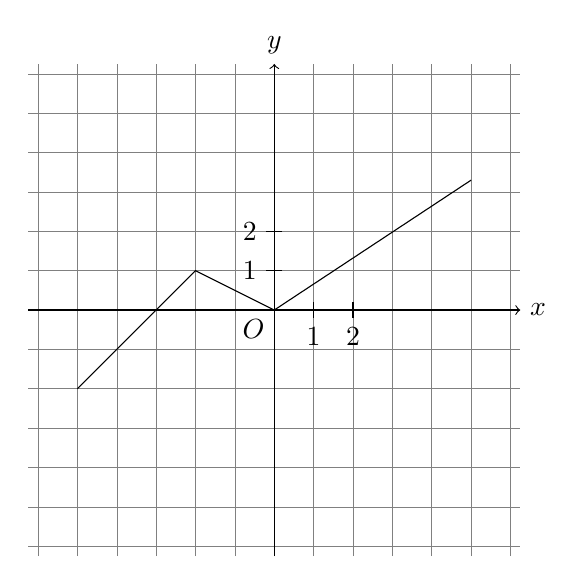
\begin{tikzpicture}[scale=0.5]
\draw[help lines] (-6.25,-6.25) grid (6.25,6.25);
\draw[->] (-6.25,0) -- (6.25,0) node[right] {$x$};
\draw[->] (0,-6.25) -- (0,6.25) node[above] {$y$};
\foreach \x in {1,2}
    {\draw (\x,0.2)--(\x,-0.2) node[below] {$\x$};}
\foreach \y in {1,2}
    {\draw (0.2,\y)--(-0.2,\y) node[left] {$\y$};}
\draw (0,0) node[below left] {$O$};

\draw (-5,-2) -- (-2,1) -- (0,0) -- (5,3.3);
\end{tikzpicture}
\end{center}
$\mathcal{S}$ = \answersline
\end{minipage}
\hfill
\begin{minipage}{0.4\textwidth}
\begin{equation*}
f(x) = -3
\end{equation*}
\begin{center}
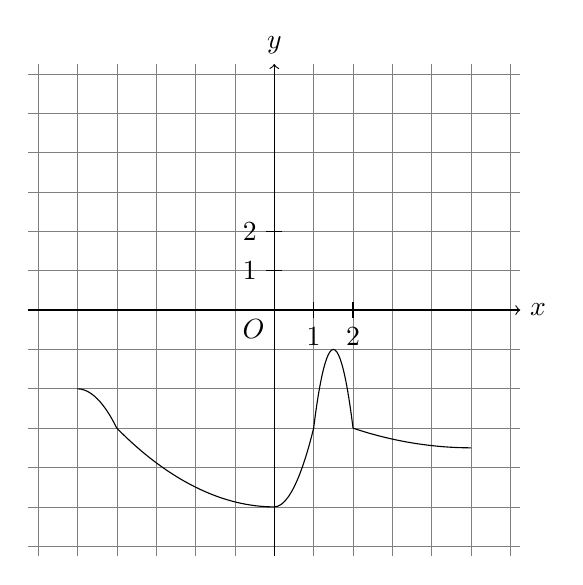
\begin{tikzpicture}[scale=0.5]
\draw[help lines] (-6.25,-6.25) grid (6.25,6.25);
\draw[->] (-6.25,0) -- (6.25,0) node[right] {$x$};
\draw[->] (0,-6.25) -- (0,6.25) node[above] {$y$};
\foreach \x in {1,2}
    {\draw (\x,0.2)--(\x,-0.2) node[below] {$\x$};}
\foreach \y in {1,2}
    {\draw (0.2,\y)--(-0.2,\y) node[left] {$\y$};}
\draw (0,0) node[below left] {$O$};

\draw (-5,-2) parabola (-4,-3);
\draw (-4,-3) parabola bend (0,-5) (1,-3);
\draw (1,-3) parabola bend (1.5,-1) (2,-3);
\draw (2,-3) parabola[bend at end] (5,-3.5);
\end{tikzpicture}
\end{center}
$\mathcal{S}$ = \answersline
\vspace*{0.5cm}
\begin{equation*}
f(x) < 1
\end{equation*}
\begin{center}
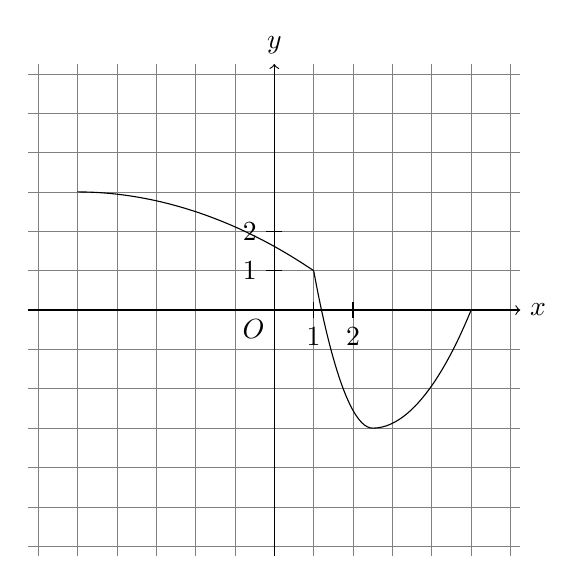
\begin{tikzpicture}[scale=0.5]
\draw[help lines] (-6.25,-6.25) grid (6.25,6.25);
\draw[->] (-6.25,0) -- (6.25,0) node[right] {$x$};
\draw[->] (0,-6.25) -- (0,6.25) node[above] {$y$};
\foreach \x in {1,2}
    {\draw (\x,0.2)--(\x,-0.2) node[below] {$\x$};}
\foreach \y in {1,2}
    {\draw (0.2,\y)--(-0.2,\y) node[left] {$\y$};}
\draw (0,0) node[below left] {$O$};

\draw (-5,3) parabola (1,1);
\draw (1,1) parabola bend (2.5,-3) (5,0);
\end{tikzpicture}
\end{center}
$\mathcal{S}$ = \answersline
\end{minipage}
\end{questions}
\end{document}